% Gemini theme
% https://github.com/anishathalye/gemini

\documentclass[final]{beamer}

% ====================
% Packages
% ====================

\usepackage[T1]{fontenc}
\usepackage{lmodern}
\usepackage[size=custom,width=120,height=72,scale=1.0]{beamerposter}
\usetheme{gemini}
\usecolortheme{minipw}
\usepackage{graphicx}
\usepackage{tikz}
\usepackage{pgfplots}
\usepackage{booktabs}
\usepackage[justification=justified,singlelinecheck=false]{subcaption}
\usepackage{multirow}  % table row span
\usepackage{siunitx}  % number formatting
\usepackage{bbm}  % math indicator
\usepackage{hyperref}  % href mailto
\usepackage{amsmath}  % math symbols

% ====================
% Lengths
% ====================

% If you have N columns, choose \sepwidth and \colwidth such that
% (N+1)*\sepwidth + N*\colwidth = \paperwidth
\newlength{\sepwidth}
\newlength{\colwidth}
\setlength{\sepwidth}{0.025\paperwidth}
\setlength{\colwidth}{0.3\paperwidth}

\newcommand{\separatorcolumn}{\begin{column}{\sepwidth}\end{column}}

% ====================
% Title
% ====================

\title{Artificial Intelligence Systems for Solving IQ Tests}

\author{Mikołaj Małkiński \\ thesis supervisor: Prof. Jacek Mańdziuk, Ph.D., D.Sc.}

\institute[shortinst]{Warsaw University of Technology, Faculty of Mathematics and Information Science}

% ====================
% Footer (optional)
% ====================

\footercontent{
Warsaw, December 2020 \hfill
Master's diploma thesis in the field of study Data Science \hfill
\href{mailto:mikolaj.malkinski@gmail.com}{mikolaj.malkinski@gmail.com}
}
% (can be left out to remove footer)

% ====================
% Logo (optional)
% ====================

% use this to include logos on the left and/or right side of the header:
% \logoright{\includegraphics[height=7cm]{images/pw.jpg}}
% \logoleft{\includegraphics[height=7cm]{logo2.pdf}}

% ====================
% Custom commands
% ====================

\newcommand{\cnnhrinet}{CNN\texttt{+}HriNet}
\newcommand{\glorehrinet}{GloRe\texttt{+}HriNet}
\newcommand{\hrinetnalu}{HriNet\texttt{+}NALU}
\newcommand{\hrinetrn}{HriNet\texttt{+}RN}
\newcommand{\hrinetpredinet}{HriNet\texttt{+}Predinet}
\newcommand{\hrinetmha}{HriNet\texttt{+}MHA}
\newcommand{\hrinetaa}{HriNet\texttt{+}AA}

\graphicspath{{../images/}}

% ====================
% Bibliography style
% ====================

\setbeamertemplate{bibliography entry article}{}
\setbeamertemplate{bibliography entry title}{}
\setbeamertemplate{bibliography entry location}{}
\setbeamertemplate{bibliography entry note}{}

% ====================
% Body
% ====================

\begin{document}

    \begin{frame}[t]
        \begin{columns}[t]
            \separatorcolumn

            \begin{column}{\colwidth}

                \begin{block}{Introduction}
                    Intelligence can be decomposed into plenty of constituting factors such as pattern recognition, ability to perform arithmetic operations or \textbf{reasoning about abstract concepts}.
                    The ability to solve abstract reasoning tasks is considered one of the hallmarks of human intelligence, which can be roughly estimated by measuring subjects' performance on \textbf{IQ tests}.
                    We focus on a specific version of such problems---the \textbf{Raven's Progressive Matrices} (RPMs)---presented in Figure~\ref{fig:rpm}.
                    \begin{figure}
                        \centering
                        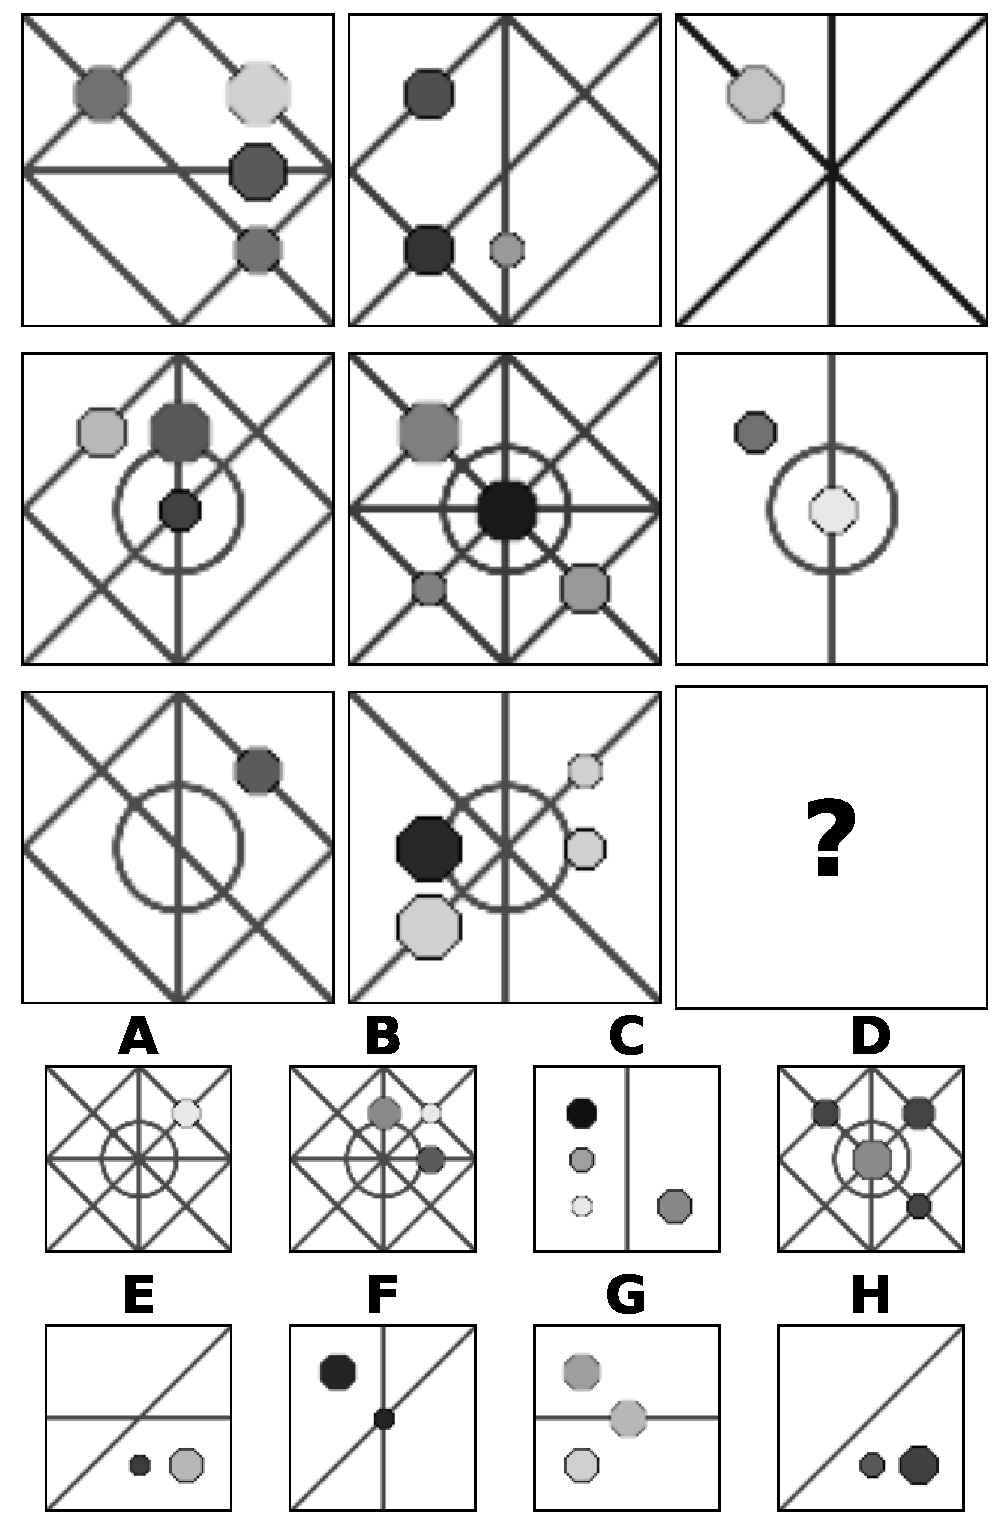
\includegraphics[width=0.31\textwidth]{pgm_rpm_0}
                        ~
                        ~
                        ~
                        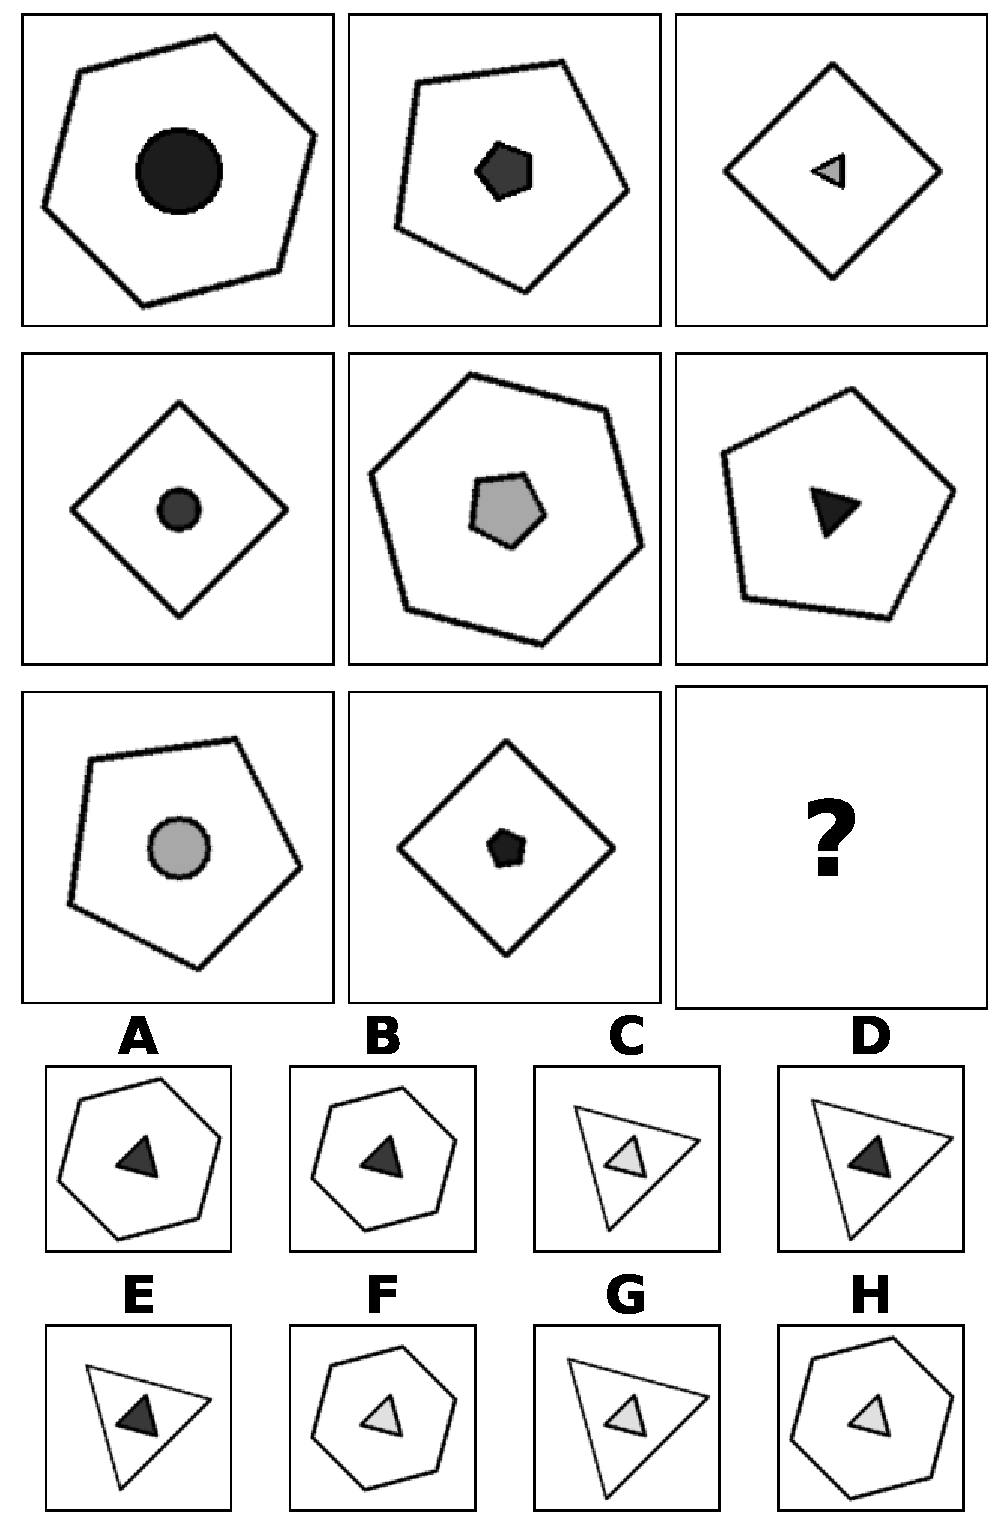
\includegraphics[width=0.31\textwidth]{raven_rpm_0}
                        \caption{
                        Solving RPMs requires to identify abstract relationships hidden behind random visual distractors and contrast possible answers to select the one which fits best.
                        Left RPM, although has more visual details, is governed by only a single rule (row-wise AND applied to shape position), whereas perceptually simpler right RPM contains 8 distinct relations applied to both outer and inner structures.
                        The examples come from the \textbf{PGM}~\cite{santoro2018measuring} and \textbf{Balanced-RAVEN}~\cite{zhang2019raven} datasets respectively.
                        In both cases the correct answer---which is to be placed in the bottom-right panel---is A.
                        }
                        \label{fig:rpm}
                    \end{figure}
                \end{block}

                \begin{block}{Augmentation of RPMs}
                    \begin{figure}[t]
                        \centering
                        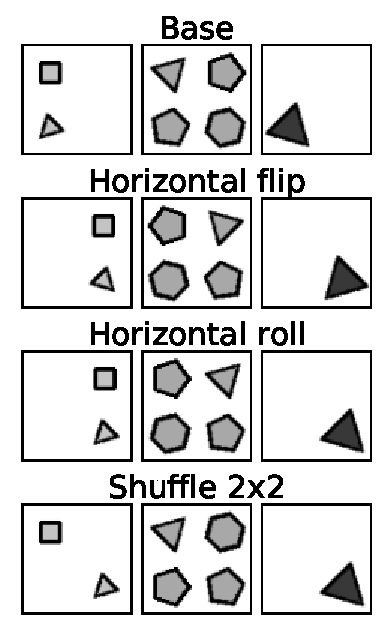
\includegraphics[width=0.29\textwidth]{augmentation_2x2}
                        ~
                        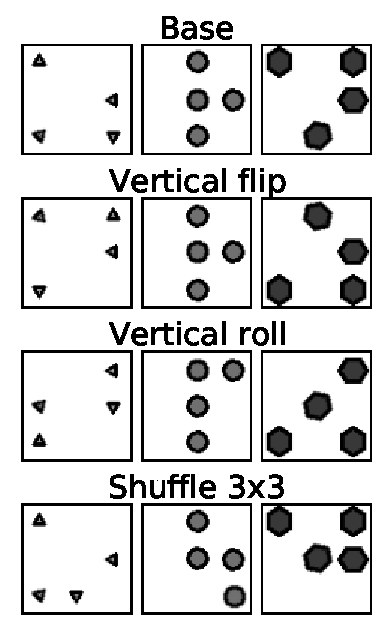
\includegraphics[width=0.29\textwidth]{augmentation_3x3}
                        \caption{
                        Augmentation of RPMs from the Balanced-RAVEN dataset.
                        Selected transformation is applied in the same way to all images in a given RPM.
                        The data augmentation module applies a randomly selected combination of presented methods with additional random rotation and transposition.
                        For clarity, we only depict different views of a single row for two RPMs belonging to configurations \texttt{2x2Grid} (left part) and \texttt{3x3Grid} (right part), respectively.
                        }
                        \label{fig:augmentation}
                    \end{figure}
                \end{block}

            \end{column}

            \separatorcolumn

            \begin{column}{\colwidth}

                \begin{block}{Neural modules}
                    In order to better understand which neural network components are useful for solving abstract relational reasoning problems, we propose and evaluate \textbf{11 new architectures} based on:
                    \begin{itemize}
                        \item \textbf{HriNet}~\cite{hu2020hierarchical}: 1) we replace the original perceptual ResNet backbone with a simpler CNN; 2) incorporate Global Reasoning units (GloRe); 3) introduce a novel rotation-based \textit{Vortex Convolution} module; combine with a variety of reasoning modules including 4) Neual Artithmetic Logic Units, 5) Relation Networks, 6) Predinet, 7) Multi-Head Attention and 8) Area Attention,
                        \item \textbf{WReN}~\cite{santoro2018measuring}: 9) we extend the relational component to handle object triplets,
                        \item \textbf{SCL}~\cite{wu2020scattering}: 10) we propose a generalized non-linear scattering transformation which considers all available group assignments and 11) a multi-head scattering operation.
                    \end{itemize}
                \end{block}

                \begin{alertblock}{Learning to solve RPMs}
                    We have considered the following methodologies of learning to solve RPMs:
                    \begin{itemize}
                        \item \textbf{Supervised} (CE) - trains the network to correctly predict index of the correct answer, by estimating the true probability distribution $p=\text{onehot}(k)$ (see \textit{Scoring} branch in Fig.~\ref{fig:mlcl}),
                        \item \textbf{Auxiliary} (AUX) - in this setup, the model has to predict an encoded representation of the abstract rules (see \textit{Rule prediction} branch in Fig.~\ref{fig:mlcl}). For this purpose we propose a novel \textbf{sparse encoding}~\cite{malkinski2020multi}, which is superior in all experiments on Balanced-RAVEN to previously used \textit{dense encoding}~\cite{santoro2018measuring,zhang2019raven}.
                        \item \textbf{Multi-Label Contrastive Learning} (MLCL) - a novel method of learning to solve RPMs which casts the problem into a \textbf{multi-label classification framework}, employs the proposed sparse encoding and introduces a \textbf{contrasting mechanism} in the objective function (see Fig.~\ref{fig:mlcl}).
                    \end{itemize}
                \end{alertblock}

                \begin{block}{Multi-Label Contrastive Learning}
                    \begin{figure}
                        \centering
                        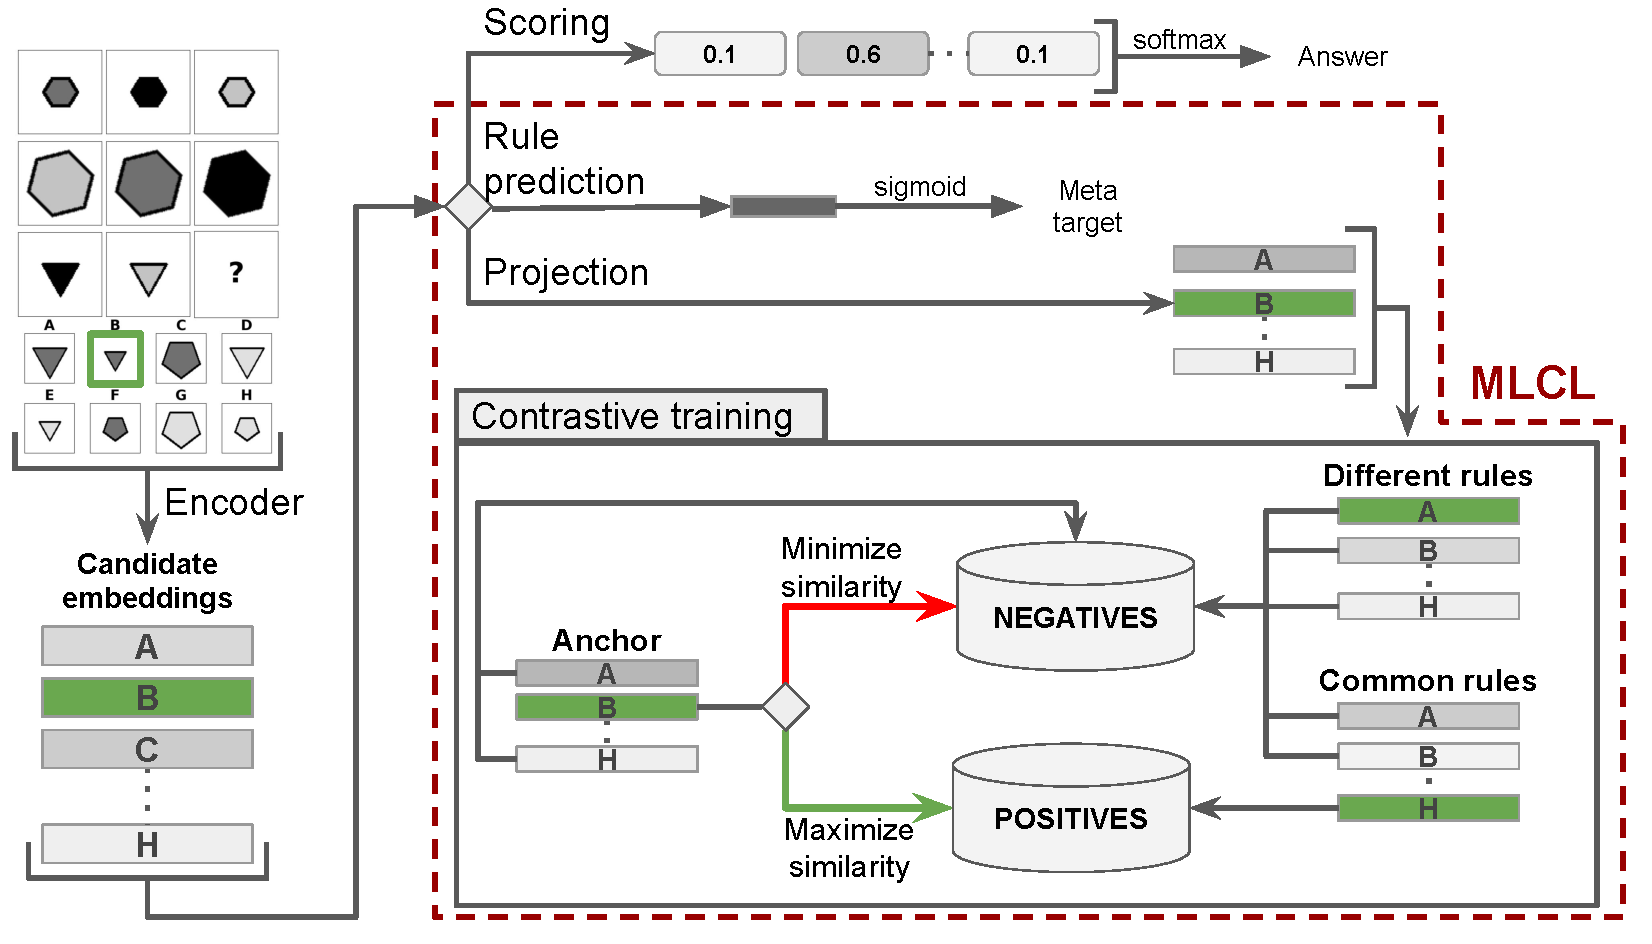
\includegraphics[width=0.8\columnwidth]{MLCL_wide}
                        \caption{
                        In each training setup we complete the context matrix with each of the choice panels and generate \textit{candidate embeddings} $h$ using an encoder network $\mathcal{N}$.
                        The candidate embedding corresponding to the answer which correctly completes the matrix is depicted in green.
                        The embeddings are processed via three different paths: 1) a scoring head $\psi$ predicts the probability distribution $\hat{p}$ of answers, 2) a rule prediction network $\rho$ estimates the underlying rules $\hat{\pi}$ as encoded meta-targets and 3) a contrastive projection network $g$ transforms them into lower-dimensional vectors $z$, which are later used for the purpose of computing the contrastive loss.
                        Both rule prediction and contrastive projection branches constitute the proposed MLCL framework.
                        }
                        \label{fig:mlcl}
                    \end{figure}
                \end{block}

            \end{column}

            \separatorcolumn

            \begin{column}{\colwidth}

                \begin{block}{Multi-Label Supervised Contrastive Loss}
                    We aim to encourage abstract reasoning models to recognise the underlying RPM rules, which are necessary to identify the correct answer.
                    Our extension of the Supervised Contrastive Loss~\cite{khosla2020supervised} for multi-label data points $\mathcal{L}^{\text{mlc}}$ minimizes the similarity of the anchor to negative samples (incorrectly completed RPMs and correctly completed RPMs with different rules) and maximizes the similarity to positive pairs (correctly completed RPMs with common rules) (see Fig.~\ref{fig:mlcl}):
                    \begin{align*}
                        \mathcal{L}^{\text{mlc}} &= \sum_{i=1}^{2N} \frac{1}{2N_{\widetilde{Y}_i} - 1} \sum_{j=1}^{2N} \mathbbm{1}_{i \neq j} \cdot \mathbbm{1}_{\widetilde{Y}_i \cap \widetilde{Y}_j \neq \emptyset} \cdot \mathcal{L}_{i,j}^{\text{mlc}}\\
                        \mathcal{L}_{i,j}^{\text{mlc}} &= - \log\frac{\exp(z_i \cdot z_j / \tau)}{\sum_{k=1}^{2N} \mathbbm{1}_{i \neq k} \cdot \exp(z_i \cdot z_k / \tau) + \mathcal{L}_{i,j,k}^{\text{mlc}}}\\
                        \mathcal{L}_{i,j,k}^{\text{mlc}} &= \sum^7_{l=1} \exp(z_i \cdot z'_{k,l} / \tau)
                    \end{align*}
                \end{block}

                \begin{block}{Main results}
                    \begin{table}[t]
                        \centering
                        \caption{
                        Test accuracy on Balanced-RAVEN averaged across 4 random seeds.
                        Each model achieves best results when trained with the proposed MLCL approach with data augmentation (DA).
                        Most notably, SCL trained with MLCL and DA sets a \textbf{new state-of-the-art} result with an absolute improvement of 1.8 p.p. over best result from the literature~\cite{wu2020scattering}.
                        }
                        \label{tab:balanced-raven}
%                        \rmfamily
                        \begin{tabular}{lc|ccc}
                            \toprule
                            \multirow{2}{*}{Method} & \multirow{2}{*}{DA} & \multicolumn{3}{c}{Mean test accuracy $\pm$ Std (\%)} \\
                            &            & SCL                     & HriNet                  & CoPINet                 \\
                            \midrule
                            \multirow{2}{*}{CE}   & \texttimes & $82.8 \pm 0.7$          & $50.6 \pm 1.3$          & $44.8 \pm 0.8$          \\
                            & \checkmark & $89.7 \pm 1.0$          & $56.7 \pm 1.6$          & $47.2 \pm 3.4$          \\
                            \midrule
                            AUX                   & \texttimes & $86.9 \pm 3.5$          & $51.6 \pm 1.5$          & $32.2 \pm 1.9$          \\
                            dense                 & \checkmark & $91.4 \pm 2.9$          & $56.7 \pm 1.2$          & $33.6 \pm 2.4$          \\
                            \midrule
                            AUX                   & \texttimes & $95.9 \pm 0.3$          & $57.0 \pm 1.6$          & $46.8 \pm 2.3$          \\
                            sparse                & \checkmark & $96.0 \pm 0.9$          & $64.2 \pm 1.2$          & $46.3 \pm 1.4$          \\
                            \midrule
                            \multirow{2}{*}{MLCL} & \texttimes & $95.7 \pm 0.5$          & $56.2 \pm 1.5$          & $57.1 \pm 0.4$          \\
                            & \checkmark & $\textbf{96.8} \pm 0.4$ & $\textbf{65.7} \pm 2.4$ & $\textbf{58.0} \pm 0.4$ \\
                            \bottomrule
                        \end{tabular}
                    \end{table}
                \end{block}

                \begin{block}{References}

                    \nocite{*}
                    \footnotesize{\bibliographystyle{plain}\bibliography{main}}

                \end{block}

            \end{column}

            \separatorcolumn
        \end{columns}
    \end{frame}

\end{document}
